\documentclass[lettersize,journal]{IEEEtran}
\usepackage{amsmath,amsfonts}
\usepackage{algorithmic}
\usepackage{array}
\usepackage[caption=false,font=normalsize,labelfont=sf,textfont=sf]{subfig}
\usepackage{textcomp}
\usepackage{stfloats}
\usepackage{url}
\usepackage{verbatim}
\usepackage{graphicx}
\hyphenation{op-tical net-works semi-conduc-tor IEEE-Xplore}
\def\BibTeX{{\rm B\kern-.05em{\sc i\kern-.025em b}\kern-.08em
    T\kern-.1667em\lower.7ex\hbox{E}\kern-.125emX}}
\usepackage{balance}
\begin{document}
\title{How to Use the IEEEtran \LaTeX \ Templates}
\author{IEEE Publication Technology Department
\thanks{Manuscript created October, 2020; This work was developed by the IEEE Publication Technology Department. This work is distributed under the \LaTeX \ Project Public License (LPPL) ( http://www.latex-project.org/ ) version 1.3. A copy of the LPPL, version 1.3, is included in the base \LaTeX \ documentation of all distributions of \LaTeX \ released 2003/12/01 or later. The opinions expressed here are entirely that of the author. No warranty is expressed or implied. User assumes all risk.}}

\markboth{Journal of \LaTeX\ Class Files,~Vol.~18, No.~9, September~2020}%
{How to Use the IEEEtran \LaTeX \ Templates}

\maketitle

\begin{abstract}
This document describes the most common article elements and how to use the IEEEtran class with \LaTeX \ to produce files that are suitable for submission to the Institute of Electrical and Electronics Engineers (IEEE).  IEEEtran can produce conference, journal and technical note (correspondence) papers with a suitable choice of class options.
\end{abstract}

\begin{IEEEkeywords}
Class, IEEEtran, \LaTeX, paper, style, template, typesetting.
\end{IEEEkeywords}


\section{Introduction}
\IEEEPARstart{W}{elcome} to the updated and simplified documentation to using the IEEEtran \LaTeX \ class file. The IEEE has examined hundreds of author submissions using this package to help formulate this easy to follow guide. We will cover the most commonly used elements of a journal article. For less common elements we will refer back to the ``IEEEtran\_HOWTO.pdf''.

This document applies to version 1.8b of IEEEtran. 

The IEEEtran template package contains the following example files: 
\begin{list}{}{}
\item{bare\_jrnl.tex}
\item{bare\_conf.tex}
\item{bare\_jrnl\_compsoc.tex}
\item{bare\_conf\_compsoc.tex}
\item{bare\_jrnl\_comsoc.tex}
\end{list}
These are ``bare bones" templates to quickly understand the document structure.  

It is assumed that the reader has a basic working knowledge of \LaTeX. Those who are new to \LaTeX \ are encouraged to read Tobias Oetiker's ``The Not So Short Introduction to \LaTeX '', available at: \url{http://tug.ctan.org/info/lshort/english/lshort.pdf} which provides an overview of working with \LaTeX.   

\section{The Design, Intent and \\ Limitations of the Templates}
\noindent The templates are intended to {\bf{approximate the final look and page length of the articles/papers}}. Therefore, {\bf{they are NOT intended to be the final produced work that is displayed in print or on IEEEXplore\textsuperscript{\textregistered}}}. They will help to give the authors an approximation of the number of pages that will be in the final version. The structure of the \LaTeX files, as designed, enable easy conversion to XML for the composition systems used by the IEEE's outsource vendors. The XML files are used to produce the final print/IEEEXplore\textsuperscript{\textregistered} pdf and then converted to HTML for IEEEXplore\textsuperscript{\textregistered}. Have you looked at your article/paper in the HTML version?

\section{\LaTeX \ Distributions: Where to Get Them}
\noindent IEEE recommends using the distribution from the \TeX User Group at \url{http://www.tug.org}. You can join TUG and obtain a DVD distribution or download for free  from the links provided on their website: \url{http://www.tug.org/texlive/}. The DVD includes distributions for Windows, Mac OS X and Linux operating systems.
 
\section{Where to get the IEEEtran Templates}
\noindent The {\bf{IEEE Template Selector}} will always have the most up-to-date versions of the \LaTeX\ and MSWord templates. Please see: \url{https://template-selector.ieee.org/} and follow the steps to find the correct template for your intended publication. Many publications use the IEEETran LaTeX templates, however, some publications have their own special templates. Many of these are  based on IEEEtran, but may have special instructions that vary slightly from those in this document.

\section{Where to get \LaTeX \ help - user groups}
\noindent The following on-line groups are very helpful to beginning and experienced \LaTeX\ users. A search through their archives can provide many answers to common questions.
\begin{list}{}{}
\item{\url{http://www.latex-community.org/}} 
\item{\url{https://tex.stackexchange.com/} }
\end{list}

\section{Document Class Options in IEEEtran}
\noindent At the beginning of your \LaTeX\ file you will need to establish what type of publication style you intend to use. The following list shows appropriate documentclass options for each of the types covered by IEEEtran.

\begin{list}{}{}
\item{Regular Journal Article}
\item{{\tt{$\backslash$documentclass[journal]{IEEEtran}}}}\\
\item{{Conference Paper}}
\item{{\tt{$\backslash$documentclass[conference]{IEEEtran}}}}\\
\item{Computer Society Journal Article}
\item{{\tt{$\backslash$documentclass[10pt,journal,compsoc]{IEEEtran}}}}\\
\item{Computer Society Conference Paper}
\item{{\tt{$\backslash$documentclass[conference,compsoc]{IEEEtran}}}}\\
\item{{Communications Society Journal Article}}
\item{{\tt{$\backslash$documentclass[journal,comsoc]{IEEEtran}}}}\\
\item{{Brief, Correspondence or Technote}}
\item{{\tt{$\backslash$documentclass[9pt,technote]{IEEEtran}}}}
\end{list}

There are other options available for each of these when submitting for peer review or other special requirements. IEEE recommends to compose your article in the base 2-column format to make sure all your equations, tables and graphics will fit the final 2-column format. Please refer to the document ``IEEEtran\_HOWTO.pdf'' for more information on settings for peer review submission if required by your EIC.

\section{How to Create Common Front Matter}
\noindent The following sections describe general coding for these common elements. Computer Society publications and Conferences may have their own special variations and will be noted below.
\subsection{Paper Title}
\noindent The title of your paper is coded as:

\begin{verbatim}
\title{The Title of Your Paper}
\end{verbatim}

\noindent Please try to avoid the use of math or chemical formulas in your title if possible.

\subsection{Author Names and Affiliations}
\noindent The author section should be coded as follows:
\begin{verbatim}
\author{Masahito Hayashi 
\IEEEmembership{Fellow, IEEE}, Masaki Owari
\thanks{M. Hayashi is with Graduate School 
of Mathematics, Nagoya University, Nagoya, 
Japan}
\thanks{M. Owari is with the Faculty of 
Informatics, Shizuoka University, 
Hamamatsu, Shizuoka, Japan.}
}
\end{verbatim}
Be sure to use the $\backslash$IEEEmembership command to identify IEEE membership status.
Please see the ``IEEEtran\_HOWTO.pdf'' for specific information on coding authors for Conferences and Computer Society publications. Note that the closing curly brace for the author group comes at the end of the thanks group. This will prevent you from creating a blank first page.

\subsection{Running Heads}
\noindent The running heads are declared by using the $\backslash${\tt{markboth}} command. There are two arguments to this command: the first contains the journal name information and the second contains the author names and paper title.
\begin{verbatim}
\markboth{Journal of Quantum Electronics, 
Vol. 1, No. 1, January 2021}
{Author1, Author2, 
\MakeLowercase{\textit{(et al.)}: 
Paper Title}
\end{verbatim}

\subsection{Copyright Line}
\noindent For Transactions and Journals papers, this is not necessary to use at the submission stage of your paper. The IEEE production process will add the appropriate copyright line. If you are writing a conference paper, please see the ``IEEEtran\_HOWTO.pdf'' for specific information on how to code "Publication ID Marks".

\subsection{Abstracts}
\noindent The abstract is the first element of a paper after the $\backslash${\tt{maketitle}} macro is invoked.  The coding is simply:
\begin{verbatim}
\begin{abstract}
Text of your abstract.
\end{abstract}
\end{verbatim}
Please try to avoid mathematical and chemical formulas in the abstract.

\subsection{Index Terms}
\noindent The index terms are used to help other researchers discover your paper. Each society may have it's own keyword set. Contact the EIC of your intended publication for this list.
\begin{verbatim}
\begin{IEEEkeywords}
Broad band networks, quality of service
\end{IEEEkeywords}
\end{verbatim}
\section{How to Create Common Body Elements}
\noindent The following sections describe common body text elements and how to code them.

\subsection{Initial Drop Cap Letter}
\noindent The first text paragraph uses a ``drop cap'' followed by the first word in ALL CAPS. This is accomplished by using the $\backslash${\tt{IEEEPARstart}} command as follows:
\begin{verbatim}
\IEEEPARstart{T}{his} is the first paragraph 
of your paper. . .
\end{verbatim}

\subsection{Sections and Subsections}
\noindent Section headings use standard \LaTeX\ commands: $\backslash${\tt{section}}, $\backslash${\tt{subsection}} and $\backslash${\tt{subsubsection}}. Numbering is handled automatically for you and varies according to type of publication. It is common to not indent the first paragraph following a section head by using $\backslash${\tt{noindent}} as follows:
\begin{verbatim}
\section{Section Head}
\noindent The text of your paragraph . . .
\end{verbatim}

\subsection{Citations to the Bibliography}
\noindent The coding for the citations are made with the \LaTeX\ $\backslash${\tt{cite}} command. This will produce individual bracketed reference numbers in the IEEE style. At the top of your \LaTeX\ file you should include:
\begin{verbatim}
\usepackage{cite}
\end{verbatim}
For a single citation code as follows:
\begin{verbatim}
see \cite{ams}
\end{verbatim}
This will display as: see \cite{ams}\\

For multiple citations code as follows:
\begin{verbatim}
\cite{ams,oxford,lacomp}
\end{verbatim}

This will display as \cite{ams,oxford,lacomp}

\subsection{Figures}
\noindent Figures are coded with the standard \LaTeX\ commands as follows:
\begin{verbatim}
\begin{figure}[!t]
\centering
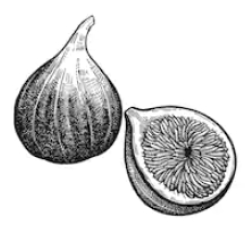
\includegraphics[width=2.5in]{fig1}
\caption{This is the caption for one fig.}
\label{fig1}
\end{figure}
\end{verbatim}
The [!t] argument enables floats to the top of the page to follow IEEE style. Make sure you include:
\begin{verbatim}
\usepackage{graphicx}
\end{verbatim}
 
\noindent at the top of your \LaTeX file with the other package declarations. 

To cross-reference your figures in the text use the following code example:
\begin{verbatim}
See figure \ref{fig1} ...
\end{verbatim}
This will produce:\\
See figure \ref{fig1} . . .

\begin{figure}[!t]
\centering
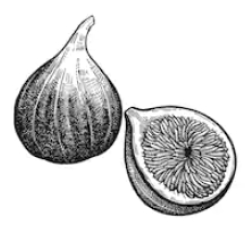
\includegraphics[width=2.5in]{fig1}
\caption{This is the caption for one fig.}
\label{fig1}
\end{figure}

\subsection{Tables}
\noindent Tables should be coded with the standard \LaTeX\ coding. The following example shows a simple table.


\begin{verbatim}
\begin{table}
\begin{center}
\caption{Filter design equations  ...}
\label{tab1}
\begin{tabular}{| c | c | c |}
\hline
Order & Arbitrary coefficients & 
coefficients\\
of filter & $e_m$ &   $b_{ij}$ \\
\hline
1& $b_{ij}=\hat{e}.\hat{\beta_{ij}}$, 
& $b_{00}=0$\\
\hline
2&$\beta_{22}=(~1,-1,-1,~~1,~~1,~~1)$ &\\ 
\hline
3& $b_{ij}=\hat{e}.\hat{\beta_{ij}}$, 
& $b_{00}=0$,\\
\hline 
\end{tabular}
\end{center}
\end{table}
\end{verbatim}
To reference the table in the text, code as follows:
\begin{verbatim}Table~\ref{tab1} lists the closed-form...\end{verbatim}
to produce:

Table~\ref{tab1} lists the closed-form . . .


%moved here for pagination purposes
\begin{table}
\begin{center}
\caption{A Simple Table Example.}
\label{tab1}
\begin{tabular}{| c | c | c |}
\hline
Order & Arbitrary coefficients & coefficients\\
of filter & $e_m$ &   $b_{ij}$ \\
\hline
1& $b_{ij}=\hat{e}.\hat{\beta_{ij}}$, & $b_{00}=0$\\
\hline
2&$\beta_{22}=(~1,-1,-1,~~1,~~1,~~1)$ &\\ 
\hline
3& $b_{ij}=\hat{e}.\hat{\beta_{ij}}$, & $b_{00}=0$,\\
\hline 
\end{tabular}
\end{center}
\end{table}


\subsection{Lists}
\noindent In this section, we will consider three types of lists: simple unnumbered, numbered and bulleted. There have been numerous options added to IEEEtran to enhance the creation of lists. If your lists are more complex than those shown below, please refer to the  ``IEEEtran\_HOWTO.pdf'' for additional options.\\

\noindent{\bf A plain  unnumbered list}

\begin{list}{}{}
\item{bare\_jrnl.tex}
\item{bare\_conf.tex}
\item{bare\_jrnl\_compsoc.tex}
\item{bare\_conf\_compsoc.tex}
\item{bare\_jrnl\_comsoc.tex}
\end{list}

\noindent coded as:
\begin{verbatim}
\begin{list}{}{}
\item{bare\_jrnl.tex}
\item{bare\_conf.tex}
\item{bare\_jrnl\_compsoc.tex}
\item{bare\_conf\_compsoc.tex}
\item{bare\_jrnl\_comsoc.tex}
\end{list}
\end{verbatim}
\noindent{\bf A simple numbered list}

\begin{enumerate}
\item{bare\_jrnl.tex}
\item{bare\_conf.tex}
\item{bare\_jrnl\_compsoc.tex}
\item{bare\_conf\_compsoc.tex}
\item{bare\_jrnl\_comsoc.tex}
\end{enumerate}
\noindent coded as: 
\begin{verbatim}
\begin{enumerate}
\item{bare\_jrnl.tex}
\item{bare\_conf.tex}
\item{bare\_jrnl\_compsoc.tex}
\item{bare\_conf\_compsoc.tex}
\item{bare\_jrnl\_comsoc.tex}
\end{enumerate}
\end{verbatim}

\noindent{\bf A simple bulleted list}

\begin{itemize}
\item{bare\_jrnl.tex}
\item{bare\_conf.tex}
\item{bare\_jrnl\_compsoc.tex}
\item{bare\_conf\_compsoc.tex}
\item{bare\_jrnl\_comsoc.tex}
\end{itemize}

\noindent coded as:

\begin{verbatim}
\begin{itemize}
\item{bare\_jrnl.tex}
\item{bare\_conf.tex}
\item{bare\_jrnl\_compsoc.tex}
\item{bare\_conf\_compsoc.tex}
\item{bare\_jrnl\_comsoc.tex}
\end{itemize}
\end{verbatim}


\subsection{Other Elements}
\noindent For other less common elements such as Algorithms, Theorems and Proofs, and Floating Structures such as page-wide tables, figures or equations, please refer to the ``IEEEtran\_HOWTO.pdf'' section on ``Double Column Floats.''


\section{How to Create Common Back Matter Elements}
\noindent The following sections demonstrate common back matter elements such as Acknowledgments, Bibliographies, Appendicies and Author Biographies.

\subsection{Acknowledgments}
\noindent This should be a simple paragraph before the bibliography to thank those individuals and institutions who have supported your work on this article.

\begin{verbatim}
\section{Acknowledgments}
\noindent Text describing those who 
supported your paper.
\end{verbatim}

\subsection{Bibliographies}
\noindent {\bf{References Simplified:}} A simple way of composing references is to use the $\backslash${\tt{bibitem}} macro to define the beginning of a reference as in the following examples:\\


\noindent [6] H. Sira-Ramirez. ``On the sliding mode control of nonlinear systems,'' \textit{Systems \& Control Letters}, vol. 19, pp. 303--312, 1992.

\noindent coded as:
\begin{verbatim}
\bibitem{Sira3}
H. Sira-Ramirez. ``On the sliding mode 
control of nonlinear systems,'' 
\textit{Systems \& Control Letters}, 
vol. 19, pp. 303--312, 1992.
\end{verbatim}

\noindent [7] A. Levant.``Exact differentiation of signals with unbounded higher derivatives,''  in \textit{Proceedings of the 45th IEEE Conference on Decision and Control}, San Diego, California, USA, pp. 5585--5590, 2006.

\noindent coded as:
\begin{verbatim}\bibitem{Levant}
A. Levant. ``Exact differentiation of 
signals with unbounded higher 
derivatives,''  in \textit{Proceedings 
of the 45th IEEE Conference on 
Decision and Control}, San Diego, 
California, USA, pp. 5585--5590, 2006.
\end{verbatim}


\noindent [8] M. Fliess, C. Join, and H. Sira-Ramirez. ``Non-linear estimation is easy,'' \textit{International Journal of Modelling, Identification and Control}, vol. 4, no. 1, pp. 12--27, 2008.

\noindent coded as:
\begin{verbatim}
\bibitem{Cedric}
M. Fliess, C. Join, and H. Sira-Ramirez. 
``Non-linear estimation is easy,'' 
\textit{International Journal of Modelling, 
Identification and Control}, vol. 4, 
no. 1, pp. 12--27, 2008.
\end{verbatim}

\noindent [9] R. Ortega, A. Astolfi, G. Bastin, and H. Rodriguez. ``Stabilization of food-chain systems using a port-controlled Hamiltonian description,'' in \textit{Proceedings of the American Control Conference}, Chicago, Illinois, USA, pp. 2245--2249, 2000.

\noindent coded as:
\begin{verbatim}
\bibitem{Ortega}
R. Ortega, A. Astolfi, G. Bastin, and H. 
Rodriguez. ``Stabilization of food-chain 
systems using a port-controlled Hamiltonian 
description,'' in \textit{Proceedings of the 
American Control Conference}, Chicago, 
Illinois, USA, pp. 2245--2249, 2000.
\end{verbatim}

\subsection{Accented Characters in References}
\noindent When using accented characters in references, please use the standard LaTeX coding for accents. {\bf{Do not use math coding for character accents}}. For example:
\begin{verbatim}
\'e, \"o, \`a, \~e 
\end{verbatim}
will produce: \'e, \"o, \`a, \~e 


\subsection{Use of BibTeX}
\noindent If you wish to use BibTeX, please see the documentation that accompanies the IEEEtran Bibliography package.

\subsection{Biographies and Author Photos}
\noindent Authors may have options to include their photo or not. Photos should be a bit-map graphic (.tif or .jpg) and sized to fit in the space allowed. Please see the coding samples below:
\begin{verbatim}
\begin{IEEEbiographynophoto}{Jane Doe}
Biography text here without a photo.
\end{IEEEbiographynophoto}
\end{verbatim}
or a biography with a photo

\begin{verbatim}
\begin{IEEEbiography}[{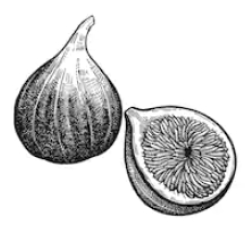
\includegraphics
[width=1in,height=1.25in,clip,
keepaspectratio]{fig1.png}}]
{IEEE Publications Technology Team} 
In this paragraph you can place 
your educational, professional background 
and research and other interests.
\end{IEEEbiography}
\end{verbatim}

Please see the end of this document to see the output of these coding examples.



\section{Mathematical Typography \\ and Why It Matters}

\noindent Typographical conventions for mathematical formulas have been developed to {\bf provide uniformity and clarity of presentation across mathematical texts}. This enables the readers of those texts to both understand the author's ideas and to grasp new concepts quickly. While software such as \LaTeX \ and MathType\textsuperscript{\textregistered} can produce aesthetically pleasing math when used properly, it is also very easy to misuse the software, potentially resulting in incorrect math display.

IEEE aims to provide authors with the proper guidance on mathematical typesetting style and assist them in writing the best possible article.

As such, IEEE has assembled a set of examples of good and bad mathematical typesetting. You will see how various issues are dealt with. The following publications have been referenced in preparing this material:

\begin{list}{}{}
\item{\emph{Mathematics into Type}, published by the American Mathematical Society}
\item{\emph{The Printing of Mathematics}, published by Oxford University Press}
\item{\emph{The \LaTeX Companion}, by F. Mittelbach and M. Goossens}
\item{\emph{More Math into LaTeX}, by G. Gr\"atzer}
\item{AMS-StyleGuide-online.pdf, published by the American Mathematical Society}
\end{list}

Further examples can be seen at \url{http://journals.ieeeauthorcenter.ieee.org/wp-content/uploads/sites/7/IEEE-Math-Typesetting-Guide.pdf}

\subsection{Display Equations}
\noindent A simple display equation example shown below uses the ``equation'' environment. To number the equations, use the $\backslash${\tt{label}} macro to create an identifier for the equation. LaTeX will automatically number the equation for you.
\begin{equation}
\label{deqn_ex1}
x = \sum_{i=0}^{n} 2{i} Q.
\end{equation}

\noindent is coded as follows:
\begin{verbatim}
\begin{equation}
\label{deqn_ex1}
x = \sum_{i=0}^{n} 2{i} Q.
\end{equation}
\end{verbatim}

To reference this equation in the text use the $\backslash${\tt{ref}} macro. 
Please see (\ref{deqn_ex1})\\
\noindent is coded as follows:
\begin{verbatim}
Please see (\ref{deqn_ex1})\end{verbatim}

\subsection{Equation Numbering}
\noindent {\bf{Consecutive Numbering:}} Equations within an article are numbered consecutively from the beginning of the
article to the end, i.e., (1), (2), (3), (4), (5), etc. Do not use roman numerals or section numbers for equation numbering.\\

\noindent {\bf{Appendix Equations:}} The continuation of consecutively numbered equations is best in the Appendix, but numbering
 as (A1), (A2), etc., is permissible.\\

\noindent {\bf{Hyphens and Periods}}: Hyphens and periods should not be used in equation numbers, i.e., use (1a) rather than
(1-a) and (2a) rather than (2.a) for sub-equations. This should be consistent throughout the article.

\subsection{Multi-line equations and alignment}
\noindent Here we show several examples of multi-line equations and proper alignments.

\noindent {\bf{A single equation that must break over multiple lines due to length with no specific alignment.}}
\begin{multline}
\text{The first line of this example}\\
\text{The second line of this example}\\
\text{The third line of this example}
\end{multline}

\noindent is coded as:
\begin{verbatim}
\begin{multline}
\text{The first line of this example}\\
\text{The second line of this example}\\
\text{The third line of this example}
\end{multline}
\end{verbatim}

\noindent {\bf{A single equation with multiple lines aligned at the = signs}}
\begin{align}
a &= c+d \\
b &= e+f
\end{align}
\noindent is coded as:
\begin{verbatim}
\begin{align}
a &= c+d \\
b &= e+f
\end{align}
\end{verbatim}

The {\tt{align}} environment can align on multiple  points as shown in the following example:
\begin{align}
x &= y & X & =Y & a &=bc\\
x' &= y' & X' &=Y' &a' &=bz
\end{align}
\noindent is coded as:
\begin{verbatim}
\begin{align}
x &= y & X & =Y & a &=bc\\
x' &= y' & X' &=Y' &a' &=bz
\end{align}
\end{verbatim}





\subsection{Subnumbering}
\noindent The amsmath package provides a {\tt{subequations}} environment to facilitate subnumbering. An example:

\begin{subequations}\label{eq:2}
\begin{align}
f&=g \label{eq:2A}\\
f' &=g' \label{eq:2B}\\
\mathcal{L}f &= \mathcal{L}g \label{eq:2c}
\end{align}
\end{subequations}

\noindent is coded as:
\begin{verbatim}
\begin{subequations}\label{eq:2}
\begin{align}
f&=g \label{eq:2A}\\
f' &=g' \label{eq:2B}\\
\mathcal{L}f &= \mathcal{L}g \label{eq:2c}
\end{align}
\end{subequations}

\end{verbatim}

\subsection{Matrices}
\noindent There are several useful matrix environments that can save you some keystrokes. See the example coding below and the output.

\noindent {\bf{A simple matrix:}}
\begin{equation}
\begin{matrix}  0 &  1 \\ 
1 &  0 \end{matrix}
\end{equation}
is coded as:
\begin{verbatim}
\begin{equation}
\begin{matrix}  0 &  1 \\ 
1 &  0 \end{matrix}
\end{equation}
\end{verbatim}

\noindent {\bf{A matrix with parenthesis}}
\begin{equation}
\begin{pmatrix} 0 & -i \\
 i &  0 \end{pmatrix}
\end{equation}
is coded as:
\begin{verbatim}
\begin{equation}
\begin{pmatrix} 0 & -i \\
 i &  0 \end{pmatrix}
\end{equation}
\end{verbatim}

\noindent {\bf{A matrix with square brackets}}
\begin{equation}
\begin{bmatrix} 0 & -1 \\ 
1 &  0 \end{bmatrix}
\end{equation}
is coded as:
\begin{verbatim}
\begin{equation}
\begin{bmatrix} 0 & -1 \\ 
1 &  0 \end{bmatrix}
\end{equation}
\end{verbatim}

\noindent {\bf{A matrix with curly braces}}
\begin{equation}
\begin{Bmatrix} 1 &  0 \\ 
0 & -1 \end{Bmatrix}
\end{equation}
is coded as:
\begin{verbatim}
\begin{equation}
\begin{Bmatrix} 1 &  0 \\ 
0 & -1 \end{Bmatrix}
\end{equation}\end{verbatim}

\noindent {\bf{A matrix with single verticals}}
\begin{equation}
\begin{vmatrix} a &  b \\ 
c &  d \end{vmatrix}
\end{equation}
is coded as:
\begin{verbatim}
\begin{equation}
\begin{vmatrix} a &  b \\ 
c &  d \end{vmatrix}
\end{equation}\end{verbatim}

\noindent {\bf{A matrix with double verticals}}
\begin{equation}
\begin{Vmatrix} i &  0 \\ 
0 & -i \end{Vmatrix}
\end{equation}
is coded as:
\begin{verbatim}
\begin{equation}
\begin{Vmatrix} i &  0 \\ 
0 & -i \end{Vmatrix}
\end{equation}\end{verbatim}

\subsection{Arrays}
\noindent The {\tt{array}} environment allows you some options for matrix-like equations. You will have to manually key the fences, but you'll have options for alignment of the columns and for setting horizontal and vertical rules. The argument to {\tt{array}} controls alignment and placement of vertical rules.

A simple array
\begin{equation}
\left(
\begin{array}{cccc}
a+b+c & uv & x-y & 27\\
a+b & u+v & z & 134
\end{array}\right)
\end{equation}
is coded as:
\begin{verbatim}
\begin{equation}
\left(
\begin{array}{cccc}
a+b+c & uv & x-y & 27\\
a+b & u+v & z & 134
\end{array} \right)
\end{equation}
\end{verbatim}

A slight variation on this to better align the numbers in the last column
\begin{equation}
\left(
\begin{array}{cccr}
a+b+c & uv & x-y & 27\\
a+b & u+v & z & 134
\end{array}\right)
\end{equation}
is coded as:
\begin{verbatim}
\begin{equation}
\left(
\begin{array}{cccr}
a+b+c & uv & x-y & 27\\
a+b & u+v & z & 134
\end{array} \right)
\end{equation}
\end{verbatim}

An array with vertical and horizontal rules
\begin{equation}
\left( \begin{array}{c|c|c|r}
a+b+c & uv & x-y & 27\\ \hline
a+b & u+v & z & 134
\end{array}\right)
\end{equation}
is coded as:
\begin{verbatim}
\begin{equation}
\left(
\begin{array}{c|c|c|r}
a+b+c & uv & x-y & 27\\
a+b & u+v & z & 134
\end{array} \right)
\end{equation}
\end{verbatim}
Note the argument now has the pipe "$\vert$" included to indicate the placement of the vertical rules.


\subsection{Cases Structures}
\noindent Many times we find cases coded using the wrong environment, i.e., {\tt{array}}. Using the {\tt{cases}} environment will save keystrokes (from not having to type the $\backslash${\tt{left}}$\backslash${\tt{lbrace}}) and automatically provide the correct column alignment.
\begin{equation*}
{z_m(t)} = \begin{cases}
1,&{\text{if}}\ {\beta }_m(t) \\ 
{0,}&{\text{otherwise.}} 
\end{cases}
\end{equation*}
\noindent is coded as follows:
\begin{verbatim}
\begin{equation*}
{z_m(t)} = 
\begin{cases}
1,&{\text{if}}\ {\beta }_m(t),\\ 
{0,}&{\text{otherwise.}} 
\end{cases}
\end{equation*}
\end{verbatim}
\noindent Note that the ``\&'' is used to mark the tabular alignment. This is important to get  proper column alignment. Do not use $\backslash${\tt{quad}} or other fixed spaces to try and align the columns. Also, note the use of the $\backslash${\tt{text}} macro for text elements such as ``if'' and ``otherwise''.

\subsection{Function Formatting in Equations}
In many cases there is an easy way to properly format most common functions. Use of the $\backslash$ in front of the function name will in most cases, provide the correct formatting. When this does not work, the following example provides a solution using the $\backslash${\tt{text}} macro.

\begin{equation*} 
  d_{R}^{KM} = \underset {d_{l}^{KM}} {\text{arg min}} \{ d_{1}^{KM},\ldots,d_{6}^{KM}\}.
\end{equation*}

\noindent is coded as follows:
\begin{verbatim}
\begin{equation*} 
 d_{R}^{KM} = \underset {d_{l}^{KM}} 
 {\text{arg min}} \{ d_{1}^{KM},
 \ldots,d_{6}^{KM}\}.
\end{equation*}
\end{verbatim}

\subsection{ Text Acronyms inside equations}
\noindent This example shows where the acronym ``MSE" is coded using $\backslash${\tt{text\{\}}} to match how it appears in the text.

\begin{equation*}
 \text{MSE} = \frac {1}{n}\sum _{i=1}^{n}(Y_{i} - \hat {Y_{i}})^{2}
\end{equation*}

\begin{verbatim}
\begin{equation*}
 \text{MSE} = \frac {1}{n}\sum _{i=1}^{n}
(Y_{i} - \hat {Y_{i}})^{2}
\end{equation*}
\end{verbatim}

\subsection{Obsolete Coding}
\noindent Avoid the use of outdated environments, such as {\tt{eqnarray}} and \$\$ math delimiters, for display equations. The \$\$ display math delimiters are left over from PlainTeX and should not be used in \LaTeX, ever. Poor vertical spacing will result.
\subsection{Use Appropriate Delimiters for Display Equations}
\noindent Some improper mathematical coding advice has been given in various YouTube\textsuperscript{TM} videos on how to write scholarly articles, so please follow these good examples:\\

For {\bf{single-line unnumbered display equations}}, please use the following delimiters: 
\begin{verbatim}\[ . . . \] or \end{verbatim} 
\begin{verbatim}\begin{equation*} . . . \end{equation*}\end{verbatim}
Note that the * in the environment name turns off equation numbering.\\

For {\bf{multiline unnumbered display equations}} that have alignment requirements, please use the following delimiters: 
\begin{verbatim}
\begin{align*} . . . \end{align*}
\end{verbatim}

For {\bf{single-line numbered display equations}}, please use the following delimiters: 
\begin{verbatim}
\begin{equation} . . . \end{equation}
\end{verbatim}

For {\bf{multiline numbered display equations}}, please use the following delimiters: 
\begin{verbatim}
\begin{align} . . . \end{align}
\end{verbatim}

\section{LaTeX Package Suggestions}
\noindent Immediately after your documenttype declaration at the top of your \LaTeX\ file is the place where you should declare any packages that are being used. The following packages were used in the production of this document.
\begin{verbatim}
\usepackage{amsmath,amsfonts}
\usepackage{algorithmic}
\usepackage{array}
\usepackage[caption=false,font=normalsize,
   labelfont=sf,textfont=sf]{subfig}
\u00sepackage{textcomp}
\usepackage{stfloats}
\usepackage{url}
\usepackage{verbatim}
\usepackage{graphicx}
\usepackage{balance}
\end{verbatim}

\section{Additional Advice}

Please use ``soft'' (e.g., \verb|\eqref{Eq}|) or \verb|(\ref{Eq})|
cross references instead of ``hard'' references (e.g., \verb|(1)|).
That will make it possible to combine sections, add equations, or
change the order of figures or citations without having to go through
the file line by line.

Please note that the \verb|{subequations}| environment in {\LaTeX}
will increment the main equation counter even when there are no
equation numbers displayed. If you forget that, you might write an
article in which the equation numbers skip from (17) to (20), causing
the copy editors to wonder if you've discovered a new method of
counting.

{\BibTeX} does not work by magic. It doesn't get the bibliographic
data from thin air but from .bib files. If you use {\BibTeX} to produce a
bibliography you must send the .bib files. 

{\LaTeX} can't read your mind. If you assign the same label to a
subsubsection and a table, you might find that Table I has been cross
referenced as Table IV-B3. 

{\LaTeX} does not have precognitive abilities. If you put a
\verb|\label| command before the command that updates the counter it's
supposed to be using, the label will pick up the last counter to be
cross referenced instead. In particular, a \verb|\label| command
should not go before the caption of a figure or a table.

Please do not use \verb|\nonumber| or \verb|\notag| inside the
\verb|{array}| environment. It will not stop equation numbers inside
\verb|{array}| (there won't be any anyway) and it might stop a wanted
equation number in the surrounding equation.

\balance

\section{A Final Checklist}
\begin{enumerate}{}{}
\item{Make sure that your equations are numbered sequentially and there are no equation numbers missing or duplicated. Avoid hyphens and periods in your equation numbering. Stay with IEEE style, i.e., (1), (2), (3) or for sub-equations (1a), (1b). For equations in the appendix (A1), (A2), etc.}. 
\item{Are your equations properly formatted? Text, functions, alignment points in cases and arrays, etc. }
\item{Make sure all graphics are included.}
\item{Make sure your references are included either in your main LaTeX file or a separate .bib file if calling the external file.}
\end{enumerate}

\begin{thebibliography}{1}

\bibitem{ams}
{\it{Mathematics into Type}}, American Mathematical Society. Online available: 

\bibitem{oxford}
T.W. Chaundy, P.R. Barrett and C. Batey, {\it{The Printing of Mathematics}}, Oxford University Press. London, 1954.

\bibitem{lacomp}{\it{The \LaTeX Companion}}, by F. Mittelbach and M. Goossens

\bibitem{mmt}{\it{More Math into LaTeX}}, by G. Gr\"atzer

\bibitem{amstyle}{\it{AMS-StyleGuide-online.pdf,}} published by the American Mathematical Society

\bibitem{Sira3}
H. Sira-Ramirez. ``On the sliding mode control of nonlinear systems,'' \textit{Systems \& Control Letters}, vol. 19, pp. 303--312, 1992.

\bibitem{Levant}
A. Levant. ``Exact differentiation of signals with unbounded higher derivatives,''  in \textit{Proceedings of the 45th IEEE Conference on Decision and Control}, San Diego, California, USA, pp. 5585--5590, 2006.

\bibitem{Cedric}
M. Fliess, C. Join, and H. Sira-Ramirez. ``Non-linear estimation is easy,'' \textit{International Journal of Modelling, Identification and Control}, vol. 4, no. 1, pp. 12--27, 2008.

\bibitem{Ortega}
R. Ortega, A. Astolfi, G. Bastin, and H. Rodriguez. ``Stabilization of food-chain systems using a port-controlled Hamiltonian description,'' in \textit{Proceedings of the American Control Conference}, Chicago, Illinois, USA, pp. 2245--2249, 2000.

\end{thebibliography}

\begin{IEEEbiographynophoto}{Jane Doe}
Biography text here without a photo.
\end{IEEEbiographynophoto}

\begin{IEEEbiography}[{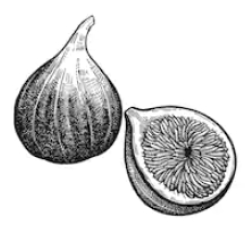
\includegraphics[width=1in,height=1.25in,clip,keepaspectratio]{fig1.png}}]{IEEE Publications Technology Team}
In this paragraph you can place your educational, professional background and research and other interests.\end{IEEEbiography}


\end{document}


